

\documentclass{article}

\usepackage{fancyhdr}
\usepackage{siunitx} % Provides the \SI{}{} and \si{} command for typesetting SI units
\usepackage{graphicx} % Required for the inclusion of images
\usepackage{natbib} % Required to change bibliography style to APA
\usepackage{amsmath} % Required for some math elements 
\usepackage[font=small,labelfont=bf]{caption}
\usepackage{float}
\setlength\parindent{0pt} % Removes all indentation from paragraphs

\usepackage{courier} %% Sets font for listing as Courier.
\usepackage{listings, xcolor}
\definecolor{myviolet}{HTML}{92268F}
\definecolor{huntergreen}{HTML}{228B22}
\lstset{
tabsize = 4, %% set tab space width
showstringspaces = false, %% prevent space marking in strings, string is defined as the text that is generally printed directly to the console
numbers = left, %% display line numbers on the left
commentstyle = \color{huntergreen}, %% set comment color
keywordstyle = \color{myviolet} \textbf, %% set keyword color
stringstyle = \color{blue}, %% set string color
rulecolor = \color{black}, %% set frame color to avoid being affected by text color
basicstyle = \small \ttfamily , %% set listing font and size
breaklines = true, %% enable line breaking
numberstyle = \tiny,
}

\pagestyle{fancy}


\bigbreak

\title{Air Traffic Controller} % Title

\author{Ingegneria del software - Progetto e sviluppo di un domain model} % Author name

\date{Niccolò \textsc{Benedetto MAT. 7024656}} % Date for the report

\begin{document}

\begin{figure}
    \centering
    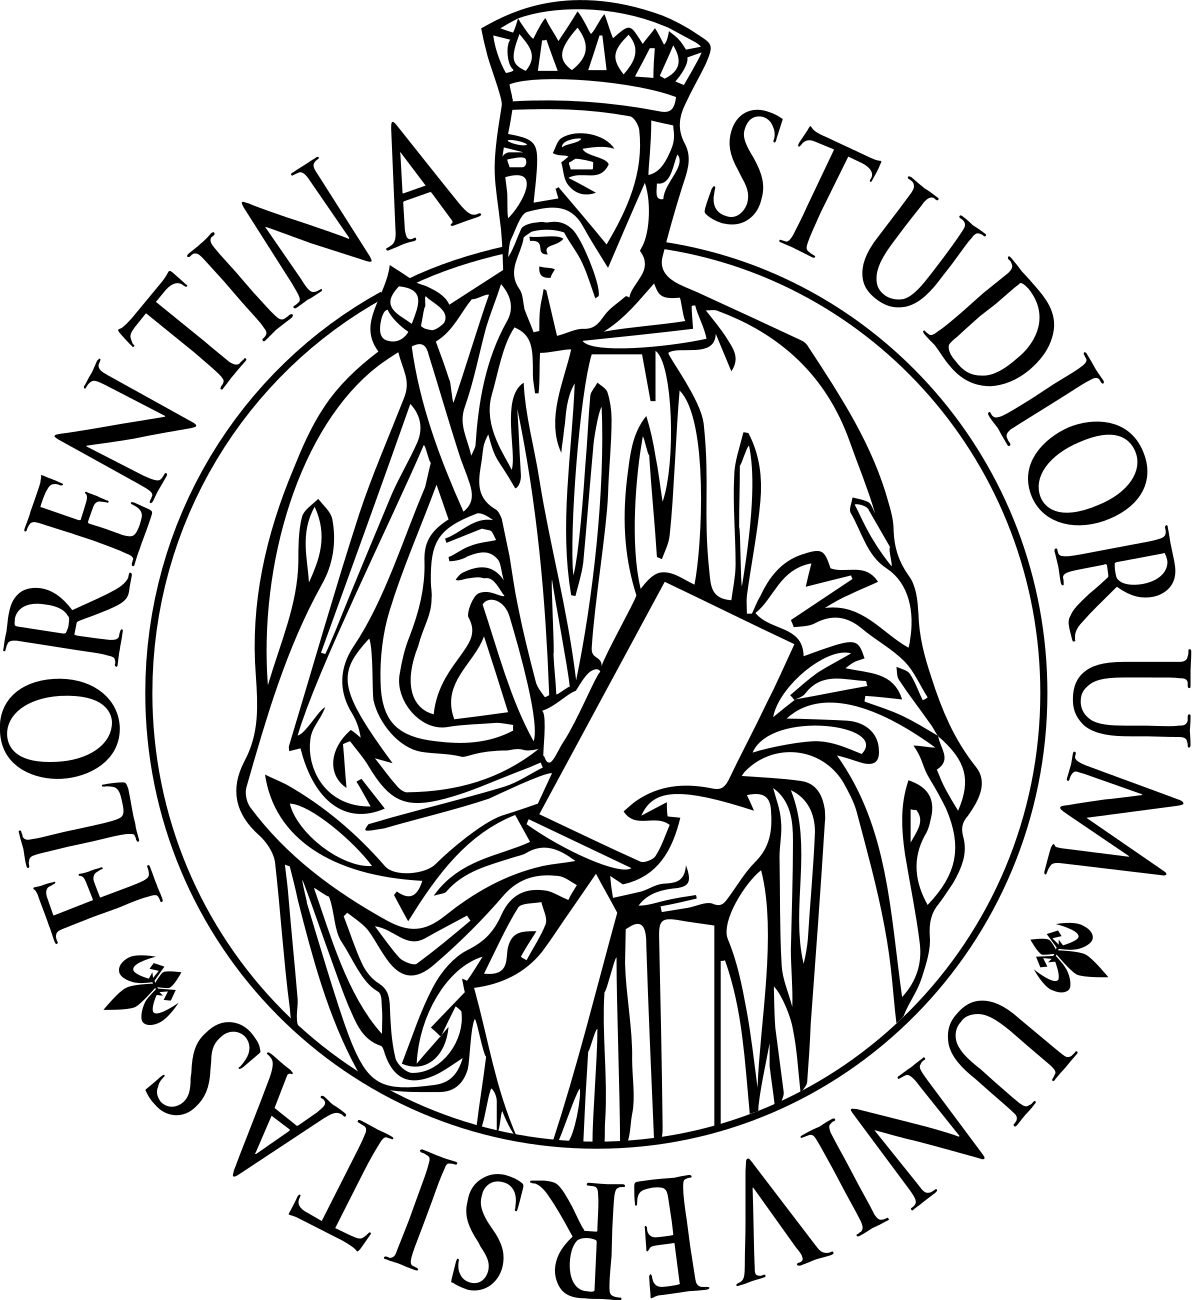
\includegraphics[scale=0.1]{Unifi_logo.png}
    \label{fig:enter-label}
\end{figure}

\maketitle

\begin{center}
\begin{tabular}{l r}
Data stesura: & Luglio 2023 \\%date 
Partners: & Takoukam Tonga Yvan \\ % Partner names

Docente: & Enrico Vicario % Instructor/supervisor
\end{tabular}
\end{center}

\newpage

\fancyhf{} % clear existing header/footer entries
% We don't need to specify the O coordinate
\fancyhead[R]{SWE domain model technical report}
\fancyfoot[C]{\thepage}

\begin{sloppy}
    

\section{Introduzione}
In questo elaborato viene posta l'attenzione sul design pattern Mediator, nonchè sul buon utilizzo di alcune pratiche dedite all'analisi, alla progettazione e 
all'implementazione di un programma JAVA e quindi di un modello di dominio \textit{well-formed}.
\bigbreak
In ingegneria del software il Mediator pattern è un design pattern utilizzato nella programmazione orientata agli oggetti che incapsula le modalità con cui oggetti diversi interagiscono fra loro.
Si tratta di un pattern comportamentale, ossia operante nel contesto delle interazioni tra oggetti, che ha l'intento di disaccoppiare entità del sistema che devono comunicare fra loro. Il pattern infatti fa in modo che queste entità non si referenzino reciprocamente, ma si riferiscano a un agente d'intermediazione, riducendo così di gran lunga il numero di interconnessioni.
Il beneficio principale consiste nel permettere la modifica agile delle politiche di interazione, poiché le entità coinvolte devono fare riferimento al loro interno solamente al mediatore. 

\bigbreak
La stesura dell'elaborato riporta:
\begin{itemize}
\item Uno scenario reale rappresentativo del modello di dominio scelto;
\item Un'analisi complessiva in cui si esplicitano i vantaggi del pattern scelto in relazione al contesto da modellare, dunque si pone l'attenzione sugli strumenti di analisi da utilizzarsi in fase di progettazione;
\item La progettazione della struttura del modello, con particolare circospezione circa i suoi partecipanti e le relazioni che tra questi sussistono;
\item Il dettaglio di frammenti di codice della realizzazione che illustrano aspetti salienti dello schema, dunque la definizione di casi di test, realizzati con \textit{JUnit}, che esercitino lo schema in uno scenario che ne caratterizza l’intento.
\end{itemize}

\section{Scenario proposto}
I piloti di veivoli che decollano dagli aereoporti non comunicano direttamente tra di loro. Questi infatti dialogano con un controllore del traffico aereo che si trova in un alta torre da qualche parte vicino alla pista. Se così non fosse ogni pilota dovrebbe conoscere le intenzioni di tutti gli altri colleghi, scaturendo non banali problematiche di comunicazione attraverso il canale radio. Dunque la torre di controllo non si occupa dell'intera tratta di volo, ma il suo compito è quello di mantenere l'ordine e organizzare i decolli di ogni veivolo.

\bigbreak

Supponiamo che nella piccola isola turistica di \textit{Lanai} (Hawaii) sia presente un aereporto dotato di due sole piste di decollo. Dalla \textit{$Runway_1$} (2500 metri) in genere decollano i voli di linea, individuati attraverso la sigla "AL" che precede il resto dell'identificatore del volo (es. "AL-001"), mentre la \textit{$Runway_2$} (2000 metri) è riservata ai private jet, il quale identifier prevede il prefisso "PJ" (es. "PJ-001"). Ogni veivolo per decollare correttamente deve in prima battuta effettuare una fase di rullaggio sulla pista assegnata dalla torre di controllo.

\bigbreak

\begin{figure}
    \centering
    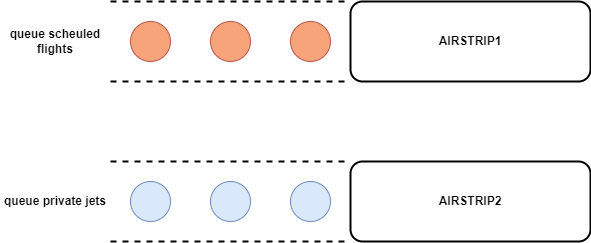
\includegraphics[scale=0.5]{figure1.png}
    \caption{proposed scenario}
    \label{fig:enter-label}
\end{figure}

\bigbreak

Le politiche aereoportuali dell'isola, affinchè sia garantita la minor congestione possibile, permettono ai piloti, in caso di code generate in fase di rullaggio, di poter fare richiesta di un cambio pista. Qualora la pista richiesta non abbia veivoli accodati il controllore del traffico aereo può soddisfare la volontà dei piloti. Segue una raffigurazione delle possibili configurazioni che si possono venire a creare.

\bigbreak

\begin{figure}[H]
    \centering
    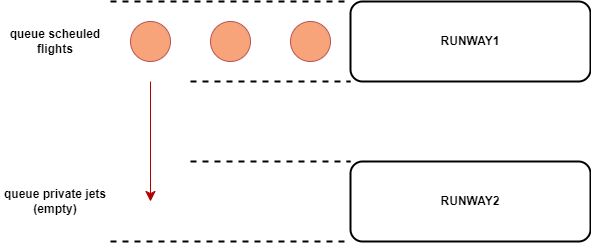
\includegraphics[scale=0.5]{figure2.png}
    \caption{a possible configuration}
    \label{fig:enter-label}
\end{figure}


\bigbreak


\begin{figure}[H]
    \centering
    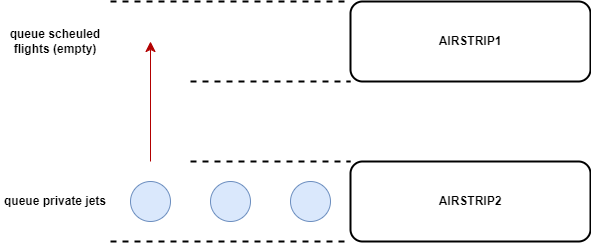
\includegraphics[scale=0.5]{figure3.png}
    \caption{a possible configuration (realistically less likely)}
    \label{fig:enter-label}
\end{figure}

\section{Analisi}
L'utilizzo del pattern Mediator permette di incapsulare il comportamento collettivo delle diverse classi che compongono il sistema (denominate \textit{colleagues} nel gergo del pattern) mediante il ricorso a una classe separata nota proprio come \textit{Mediator}, che diviene quindi quel famoso agente d'intermediazione tra i diversi oggetti.

\bigbreak

\begin{figure}[H]
    \centering
    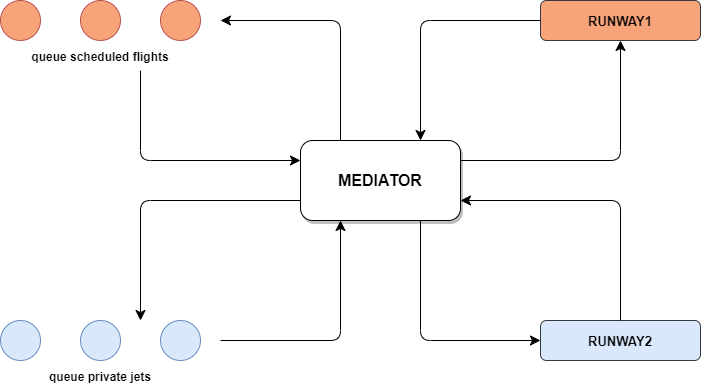
\includegraphics[scale=0.4]{figure4.png}
    \caption{Mediator logic}
    \label{fig:enter-label}
\end{figure}

\bigbreak
\bigbreak

Di seguito si definisce il sistema pattern Mediator, a cui viene fatto fede in fase di progettazione del prospetto da realizzare, quindi si elargisce una breve descrizione di ogni classe che compone lo schema. La notazione utilizzata è da ricercarsi nel linguaggio visivo dedito alla specifica, costruzione e documentazione di artefatti di sistema conosciuto come UML. 

\bigbreak
\bigbreak

\begin{figure}[H]
    \centering
    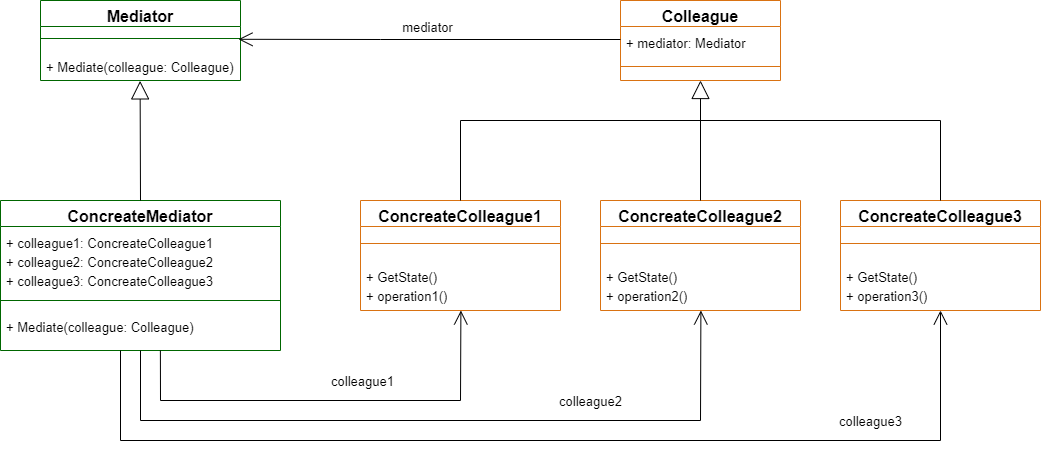
\includegraphics[scale=0.32]{figure5.png}
    \caption{UML Mediator pattern}
    \label{fig:enter-label}
\end{figure}

\bigbreak

\begin{description}
    \item[Mediator]Definisce un'interfaccia per la comunicazione tra i colleague objects.
    \item[ConcreateMediator]Implementa l'interfaccia definita dal Mediator, quindi mantiene la lista dei colleague objects e coordina lo scambio dei messaggi tra questi.
    \item[Colleague]Definisce la classe astratta (o l'interfaccia) dei colleague objects.
    \item[ConcreateColleague]Implementa le funzioni presentate nella classe \textit{Colleague}. In uno scenario realistico ce ne possono essere di tanti tipi diversi.
\end{description}

\bigbreak


\begin{figure}[H]
    \centering
    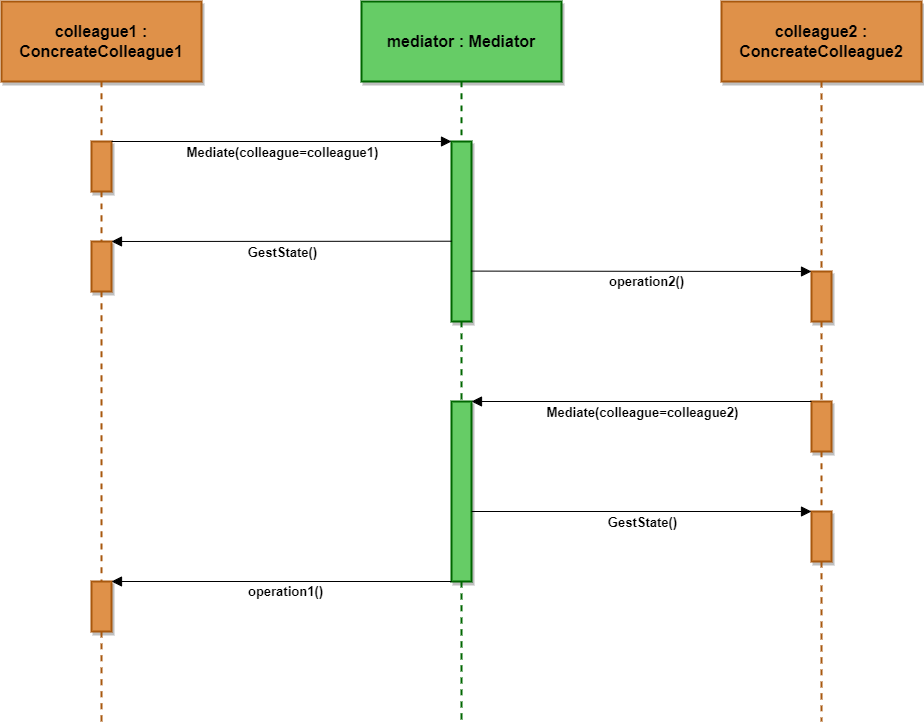
\includegraphics[scale=0.37]{figure6.png}
    \caption{Sequence diagram Mediator}
    \label{fig:enter-label}
\end{figure}

\bigbreak

Il sequence diagram è un tipo di diagramma appartenente sempre all'\textit{Unifed Modeling Language} (UML) che mostra sostanzialmente come gli "attori" del sistema si scambiano le informazioni in un ordine particolare. Si tenga presente infatti che in un sistema vengono costantemente effettuate richieste e inviate risposte. Il destinatario prende una decisione in base alla richiesta specifica e alle sue regole predeterminate. Una simile rete di possibli decisioni e interazioni (conosciuta come \textit{Activity Diagram}) assume le sembianze di un albero fortemente ramificato, ed è direttamente ottenuto a sua volta da un altro particolare artefatto denominato \textit{Use Cases Diagram}, che pone l'attenzione appunto sugli "attori" e sulle attività del sistema di cui questi si fanno carico. Il sequence diagram non rappresenta altro che un percorso specifico all'interno di questa rete, rete che quindi definisce una modalità di analisi degli \textit{Uses cases}.
Per cui un tale strumento supporta l'analisi logica per sottosezioni di sistemi, ma perde di valore se utilizzato per rappresentare l'intero apparato.
Il sequence diagram sopra riportato definisce uno scenario di test puramente dimostrativo per il pattern Mediator.
Si tenga presenta che l'elaborato debba riportare in maniera rigorosa nella sezione di Progettazione un \textit{Use Case Diagram} suggestivo del sistema e il rispettivo \textit{Activity Diagram}.



\bigbreak
Si riassumano adesso i vantaggi derivanti dall'utilizzo del pattern Mediator in un tale scenario:
\begin{itemize}
    \item \underline{Disaccoppiamento dei colleagues}: i colleagues dialogano tra loro passando esclusivamente per il Mediator. Questo permette di poter rimpiazzare un object nella struttura creata con un object differente senza influenzare le classi definite;
    \item \underline{Semplificazione delle connessioni}: il Mediator permette di ridurre le connessioni dei colleagues da \textit{many-to-many} a \textit{one-to-many}. Si osservi che però, all'aumentare progressivo dei colleagues, il Mediator diviene più complesso e quindi aumentano le difficoltà del suo mantenimento;
    \item \underline{Controllo centralizzato}: il controllo delle comunicazioni è centralizzato, per cui si ha una visione complessiva del sistema e una gestione più efficiente delle modifiche.
    \item \underline{Subclassing ridotto}:  partendo dal presupposto che l'intera logica dello schema è incapsulata nel Mediator, qualora volessi aggiungere una dipendenza a una classe, bisognerà solamente espandere la Mediator class. Quindi in generale non è necessaria la realizzazione di subclasses.
\end{itemize}

Si osservi tuttavia che realizzando una tale struttura concettuale, si espone l'intero sistema a un \textit{single point of failure}: nel caso di malfunzionamento del Mediator l'apparato complessivo sarà coinvolto con conseguente isolamento di ogni colleague.

\section{Progettazione e Codice}

Nel sistema sono presenti 7 classi principali (di cui due di queste adempiono al mero compito di definire una prova di test del sistema puramente dimostrativa; queste classi sono riconoscibili mediante il prefisso \textit{Test}, ma è stato scelto di non rappresentarle all'interno del modello UML col fine di porre l'attenzione maggiormente sulla struttura realizzativa del sistema e non sul suo collaudo). L'interazione tra queste emula il comportamento presentato dal pattern Mediator. Per il corretto funzionamento di tutto il sistema, è necessaria una stretta collaborazione tra le varie classi, ognuna delle quali ha delle responsabilità a cui non si può sottrarre. Si è data particolare importanza ai modificatori di visibilità, per garantire che nessuna classe possa eseguire operazioni che non le sono permesse. Inoltre si è pensato di racchiudere tutte le classi all'interno di uno stesso package denominato \textit{designmodel.mediator}. Segue la modelizzazione UML del sistema.

\bigbreak
\begin{figure}[H]
    \centering
    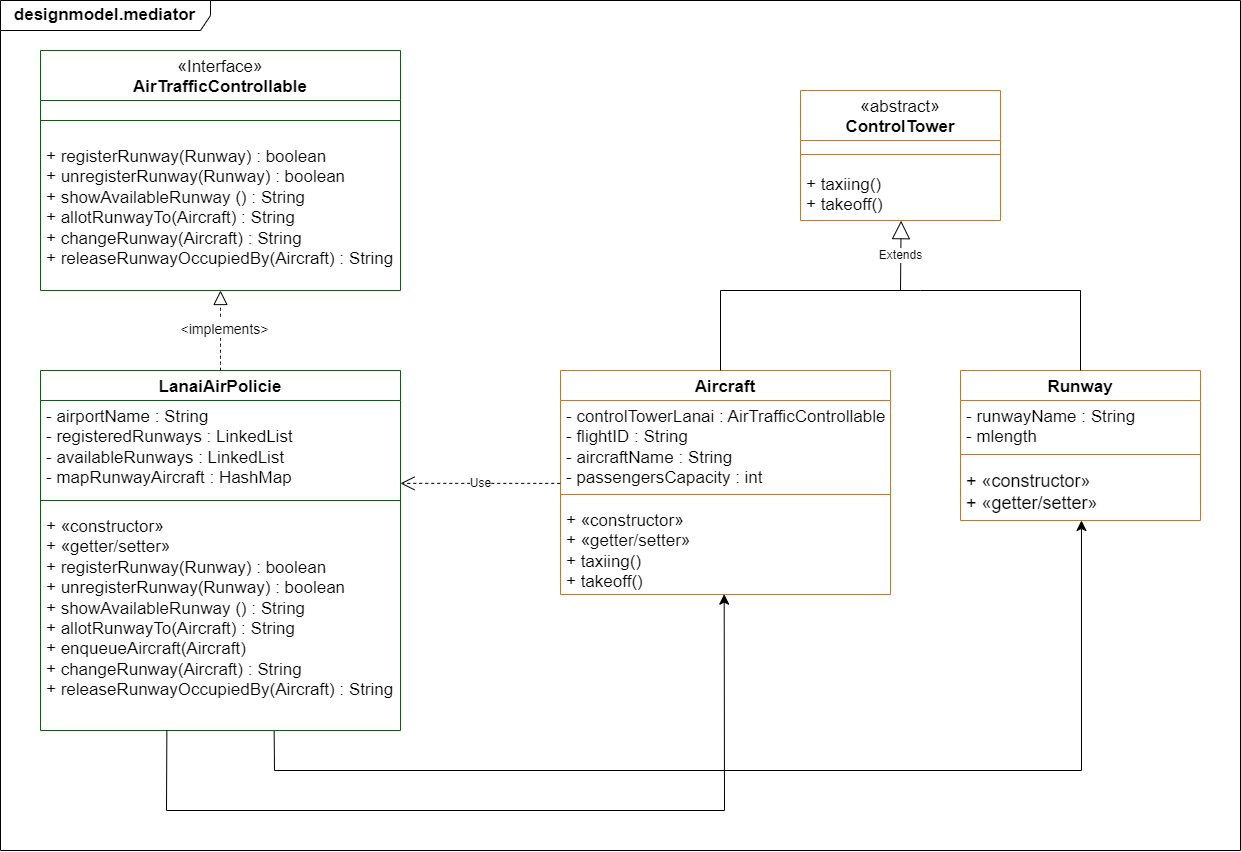
\includegraphics[scale=0.275]{figure7.png}
    \caption{UML}
    \label{fig:enter-label}
\end{figure}
\bigbreak


\begin{description}
    \item[AirTrafficControllable]Interfaccia che definisce una serie di funzionalità concretizzate da una torre di controllo, circoscritte allo scenario scelto. Nell'UML del pattern rappresenta proprio la classe \textit{Mediator}.
    \item[LanaiAirPolicie]Implementa concretamente le funzionalità introdotte nell'interfaccia tenendo come riferimento le regole e i limiti imposti dal modello. Qui viene ad esempio attuata la logica necessaria per ridurre la congestione del traffico aereo generato dalle attese passive dei veivoli che devono decollare, attraverso il metodo \textit{changeRunway()}. Tale classe assume dunque il ruolo della classe \textit{ConcreateMediator}.
    \item[ControlTower]Classe astratta che assume il ruolo di \textit{Colleague} e quindi definisce i servizi offerti ai \textit{ConcreateColleague}. Permette l'interfacciamento con quanto presentato attraverso il \textit{ConcreateMediator}. L'utilizzo di una classe astratta e non di un'interfaccia è favorito dal fatto di non avere l'obbligo di implementazione dei metodi qui fissati dentro tutti i \textit{ConcreateCollegue}. Nella progettazione delle relazioni dei partecipanti del modello caratterizzante preso come riferimento, questo vincolo deve essere rispettato. 
    \item[Aircraft]E' uno dei \textit{ConcreateColleague} del nostro modello. Rappresenta uno dei due tipi di veivoli definiti nello scenario. Implementa i metodi del \textit{ConcreateColleague}.
    \item[Runway]E' l'altro \textit{ConcreateColleague} del modello. Presenta un pezzo del sistema fondamentale per il corretto funzionamento dei metodi delle classi sopra descritte.
    \item[TestManagementRunway]Classe che sfrutta il framework \textit{JUnit 4} per testare la corretta gestione delle piste di decollo.
    \item[TestLanaiAirPolicieLogic]Classe che sfrutta il framework \textit{JUnit 4} per testare la logica presentata nella sezione 2 dell'elaborato.
\end{description}

Vengono adesso riportati alcuni frammenti di codice suggestivi del programma JAVA realizzato, organizzati per classe.

\bigbreak

\begin{lstlisting}[language = Java , frame = single , firstnumber = last , escapeinside={(*@}{@*)}]
public interface AirTrafficControllable {

	public boolean registerRunway(Runway runway);
	
	public boolean unregisterRunway(Runway runway);
	
	public String showAvailableRunway();
	
	public String allotRunwayTo(Aircraft aircraft);
	
	public String changeRunway(Aircraft aircraft);
	
	public String releaseRunwayOccupiedBy(Aircraft aircraft);
	
}

\end{lstlisting}

\begin{lstlisting}[language = Java , frame = single , firstnumber = last , escapeinside={(*@}{@*)}]
public class LanaiAirPolicie implements AirTrafficControllable{

	private String airportName;
	private LinkedList<Runway> registeredRunways = new LinkedList<>();
	private LinkedList<Runway> availableRunways = new LinkedList<>();
	private HashMap<Aircraft, Runway> mapRunwayAircraft = new HashMap<>();
	
	
	public LanaiAirPolicie(String airportName) {
		this.airportName = airportName;
	}
	
	
	public String getAirportName() {
		return airportName;
	}


	public void setAirportName(String airportName) {
		this.airportName = airportName;
	}

	@Override
	public boolean registerRunway(Runway runway) {
		
		boolean alreadyRegistered = false;
		boolean registerOutcome = false;
		
		for(Runway registeredRunway : registeredRunways) {
			if(registeredRunway.equals(runway)) {
				alreadyRegistered = true;
			}
		}
		
		if(!alreadyRegistered) {
			this.registeredRunways.add(runway);
			this.availableRunways.add(runway);
			registerOutcome = true;
		}
		
		return registerOutcome;
	}

	@Override
	public boolean unregisterRunway(Runway runway) {
		
		boolean unregisterOutcome = false;
		
		for(Runway registeredRunway : this.registeredRunways) {
			if(registeredRunway.equals(runway)) {
				unregisterOutcome = true;
				this.registeredRunways.remove(runway);
				this.availableRunways.remove(runway);
			}
		}
		
		return unregisterOutcome;
	}

	@Override
	public String showAvailableRunway() {
		
		String runwayList = "no-one available runway";
		
		if(!availableRunways.isEmpty()) {
			
			runwayList = "|";
			
			for(Runway runway : this.availableRunways) {
				runwayList = runwayList + runway.getRunwayName() + "|";
			}
			
		}
		
		return runwayList;
	}

	@Override
	public String allotRunwayTo(Aircraft aircraft) {
		
		String allotRunway = null;
		
		if(!this.availableRunways.isEmpty()) {
			
			for(Runway runway : this.availableRunways) {
				
				if(runway.getRunwayName().equals("Runway1") && 
						aircraft.getFlighID().substring(0,2).equals("AL")) {
					
					//allot proper runway to scheduled flights
					
					allotRunway = runway.getRunwayName();
					this.mapRunwayAircraft.put(aircraft, runway);
					this.availableRunways.remove(runway);
					
				}
				
				if(runway.getRunwayName().equals("Runway2") && 
						aircraft.getFlighID().substring(0,2).equals("PJ")) {
					
					//allot proper runway to private jets
					
					allotRunway = runway.getRunwayName();
					this.mapRunwayAircraft.put(aircraft, runway);
					this.availableRunways.remove(runway);
					
				}
				
			}
			
		}
		
		if(!this.mapRunwayAircraft.containsKey(aircraft)) {
			
			//there have to be a queue for some aircraft			
			enqueueAircraft(aircraft);
		}
		
		return allotRunway;
	}

	public void enqueueAircraft(Aircraft aircraft) {
		
		for(Runway runway : this.registeredRunways) {
			
			if(runway.getRunwayName().equals("Runway1") 
					&& aircraft.getFlighID().substring(0,2).equals("AL")) {
				
				//scheduled flights have to be enqueue to the Runway1
				
				this.mapRunwayAircraft.put(aircraft, runway);
				break;
				
			}
			
			if(runway.getRunwayName().equals("Runway2") 
					&& aircraft.getFlighID().substring(0,2).equals("PJ")) {
				
				//private jets have to be enqueue to the Runway2
				
				this.mapRunwayAircraft.put(aircraft, runway);
				break;
				
			}
			
		}
		
	}
	
	@Override
	public String changeRunway(Aircraft aircraft) {

		int scheduledFlightEnqueued = 0;
		int privateJetsEnqueued = 0;

		String newRunway = null;
  

		for (Aircraft enqueuedAircraft : this.mapRunwayAircraft.keySet()) {
			
			if (enqueuedAircraft.getFlighID().substring(0, 2).equals("AL")
					&& this.mapRunwayAircraft.get(enqueuedAircraft).
					getRunwayName().equals("Runway1")) {
				
				//we have to count how many scheduled flights are enqueued
				
				scheduledFlightEnqueued++;
			}
   
			if (enqueuedAircraft.getFlighID().substring(0, 2).equals("PJ")
					&& this.mapRunwayAircraft.get(enqueuedAircraft).
					getRunwayName().equals("Runway2")) {
				
				//we have to count how many private jets are enqueued
				
				privateJetsEnqueued++;
			}

		}

		if (aircraft.getFlighID().substring(0, 2).equals("AL") && 
				scheduledFlightEnqueued > 1 && privateJetsEnqueued == 0) {

			//scenario for changing runway for scheduled flights
			
			for (Runway runway : this.availableRunways) {
				if (runway.getRunwayName().equals("Runway2")) {
					this.mapRunwayAircraft.put(aircraft, runway);
					this.availableRunways.remove(runway);
					newRunway = runway.getRunwayName();
				}
			}

		}

		if (aircraft.getFlighID().substring(0, 2).equals("PJ") && 
				scheduledFlightEnqueued == 0 && privateJetsEnqueued > 1) {

			//scenario for changing runway for private jets
			
			for (Runway runway : this.availableRunways) {
				if (runway.getRunwayName().equals("Runway1")) {
					this.mapRunwayAircraft.put(aircraft, runway);
					this.availableRunways.remove(runway);
					newRunway = runway.getRunwayName();
				}
			}

		}

		return newRunway;
	}

	@Override
	public String releaseRunwayOccupiedBy(Aircraft aircraft) {

		String releasedRunway = null;
  
		boolean alreadyAvailable = false;

		for (Runway runway : this.availableRunways) {

			if (runway.equals(this.mapRunwayAircraft.get(aircraft))) {

				alreadyAvailable = true;

			}

		}

		if (!alreadyAvailable) {
			this.availableRunways.add(this.mapRunwayAircraft.get(aircraft));
		}

		releasedRunway = this.mapRunwayAircraft.get(aircraft).getRunwayName();

		return releasedRunway;
	}

}


\end{lstlisting}

\begin{lstlisting}[language = Java , frame = single , firstnumber = last , escapeinside={(*@}{@*)}]
public class Aircraft
{

    private AirTrafficControllable controlTower;

    public void taxxing() {

		
		System.out.println("Available runways: " + this.controlTower.
				showAvailableRunway());
		
		String allotAirstrip = this.controlTower.allotRunwayTo(this);
		
		if(!Objects.isNull(allotAirstrip)) {
			
			
			System.out.println(this.aircraftName + "'s [" + this.flighID + "]" + 
					" taxxing on the " + allotAirstrip);
			
			System.out.println("Available runways: " + this.controlTower.
					showAvailableRunway());
			
			
		}else {
			
			System.out.println(this.aircraftName + " [" + this.flighID + "] can't taxi" );
			
			System.out.println(this.aircraftName + " [" + this.flighID + "] requests "
					+ "the control tower for a runway change" );
			
			String newRunway = this.controlTower.changeRunway(this);
			
			if(!Objects.isNull(newRunway)) {
				
				System.out.println("Control tower confirms the request and it allot " 
				+ newRunway + " to [" + this.flighID + "]");
				
				System.out.println("Available runways: " + 
						this.controlTower.showAvailableRunway());
				
			}else {
				
				System.out.println("Control tower denys the requests because all the "
						+ "runways are not available");
				
			}
			

		}
		
    }

    public void takeoff() {
		
		String releasedAirstrip = this.controlTower.releaseRunwayOccupiedBy(this);
		
		if(!Objects.isNull(releasedAirstrip)) {
			
			System.out.println(this.aircraftName + " [" + this.flighID + "] take off "
					+ "correctly from " + releasedAirstrip);
			
			System.out.println("Availble runways: " + this.controlTower.showAvailableRunway());
			
			
		}
		
    }
   
}



\end{lstlisting}

\bigbreak

Supponendo di aver un blocco di 4 veivoli, composto da 3 scheduled flights (voli di linea) e 1 private jet, che richiedono il rullaggio (taxi) necessario per il corretto decollo nel seguente ordine:
\begin{enumerate}
    \item $scheduled fligth_1$
    \item $scheduled fligth_2$
    \item $private jet_1$
    \item $scheduled fligth_3$
\end{enumerate}

Allora, implementando la logica presentata, vorremmo che il programma rispondesse come di seguito riportato.

\bigbreak
\begin{lstlisting}[language =  , frame = single , firstnumber = last , escapeinside={(*@}{@*)}]
Available runways: |Runway1|Runway2|
Airbus480's [AL-001] taxiing on the Runway1
Available runways: |Runway2|
***************************************************************
***************************************************************
Available runways: |Runway2|
Ryanair370 [AL-002] can't taxi
Ryanair370 [AL-002] requests the control tower for a runway change
Control tower confirms the request and it allots Runway2 to [AL-002]
Available runways: no-one available runway
***************************************************************
***************************************************************
Available runways: no-one available runway
TurboJet2.0 [PJ-001] can't taxi
TurboJet2.0 [PJ-001] requests the control tower for a runway change
Control tower denys the requests because all the runways are not available
***************************************************************
***************************************************************
Available runways: no-one available runway
EasyJet [AL-003] can't taxi
EasyJet [AL-003] requests the control tower for a runway change
Control tower denys the requests because all the runways are not available
***************************************************************
***************************************************************
Airbus480 [AL-001] take off correctly from Runway1
Availble runways: |Runway1|
***************************************************************
***************************************************************
Ryanair370 [AL-002] take off correctly from Runway2
Availble runways: |Runway1|Runway2|
***************************************************************
***************************************************************
TurboJet2.0 [PJ-001] take off correctly from Runway2
Availble runways: |Runway1|Runway2|
***************************************************************
***************************************************************
EasyJet [AL-003] take off correctly from Runway1
Availble runways: |Runway1|Runway2|
***************************************************************

\end{lstlisting}

\bigbreak
L'output ottenuto deriva da una serie di stampe a video riportate in una classe contenente il metodo principale \textbf{\textit{public static void main(String[] args)}} e la sua funzione è prettamente dimostrativa.
I reali test infatti vengono eseguiti attraverso l'utilizzo del framework \textit{JUnit4}. Di seguito si è riportato un frammento di codice caratterizzante di alcune classi di test.
\bigbreak

\begin{lstlisting}[language = Java , frame = single , firstnumber = last , escapeinside={(*@}{@*)}]
public class TestLanaiAirPolicieLogic {


	private AirTrafficControllable controlTower;
	
	private Runway runway1;
	private Runway runway2;
	
	private Aircraft scheduledFlight1;
	private Aircraft scheduledFlight2;
	private Aircraft scheduledFlight3;
	private Aircraft pjet1;

	@Before
	public void setUp() throws Exception {
		
		controlTower = new LanaiAirPolicie("LANAI-airport");

		runway1 = new Runway("Runway1", 2500);
		runway2 = new Runway("Runway2", 2000);
		
		scheduledFlight1 = new Aircraft(controlTower, "AL-001", "Airbus480", 200);
		scheduledFlight2 = new Aircraft(controlTower, "AL-002", "Ryanair370", 150);
		scheduledFlight3 = new Aircraft(controlTower, "AL-003", "EasyJet", 130);
	
		pjet1 = new Aircraft(controlTower, "PJ-001", "TurboJet2.0", 20);		
		assertNotNull(controlTower);
		
		assertNotNull(runway1);
		assertNotNull(runway2);
		
		assertNotNull(scheduledFlight1);
		assertNotNull(scheduledFlight2);
		assertNotNull(scheduledFlight3);
		assertNotNull(pjet1);
		
		assertEquals(true, controlTower.registerRunway(runway1));

		assertEquals("|Runway1|", controlTower.showAvailableRunway());

		assertEquals(true, controlTower.registerRunway(runway2));

		assertEquals("|Runway1|Runway2|", controlTower.showAvailableRunway());

		
	}

	@Test
	public void testFirstBlockAircraft() {
		
		//We suppose that the first block of aircrafts arrive 
            //with the following order
		// - scheduled flight_1
		// - scheduled flight_2
		// - private jet_1
		// - scheduledflight_3
		
		
		//---------------------------------------------------
		//taxiing
		
		assertEquals("|Runway1|Runway2|", controlTower.showAvailableRunway());
		
		assertEquals("Runway1", controlTower.allotRunwayTo(scheduledFlight1));
		
		assertEquals("|Runway2|", controlTower.showAvailableRunway());
		
		assertEquals(null, controlTower.allotRunwayTo(scheduledFlight2));
		
		assertEquals("Runway2", controlTower.changeRunway(scheduledFlight2));
		
		assertEquals("no-one available runway", controlTower.showAvailableRunway());
		
		assertEquals(null, controlTower.allotRunwayTo(pjet1));
		
		assertEquals(null, controlTower.changeRunway(pjet1));
		
		assertEquals(null, controlTower.allotRunwayTo(scheduledFlight3));
		
		assertEquals(null, controlTower.changeRunway(scheduledFlight3));
		
		//---------------------------------------------------
		
		//---------------------------------------------------
		//take off
		
		assertEquals("Runway1", controlTower.releaseRunwayOccupiedBy(scheduledFlight1));
		
		assertEquals("|Runway1|", controlTower.showAvailableRunway());
		
		assertEquals("Runway2", controlTower.releaseRunwayOccupiedBy(scheduledFlight2));
		
		assertEquals("|Runway1|Runway2|", controlTower.showAvailableRunway());
		
		assertEquals("Runway2", controlTower.releaseRunwayOccupiedBy(pjet1));
		
		assertEquals("Runway1", controlTower.releaseRunwayOccupiedBy(scheduledFlight3));
		
		//---------------------------------------------------
	}

}



\end{lstlisting}

\bigbreak

Di seguito si è riportato lo \textit{Use Case Diagram} associato al programma con l'intento di catturare ulteriormente il comportamento atteso dal sistema in termini di servizi, compiti e funzioni, garantendo una visione d'insieme relazionale tra "attori" e obiettivi.
Nel diagramma è presente anche un caso d'uso, non esplicitamente richiesto nel testo del modello, che riguarda la gestione delle piste di decollo da parte dell'aereoporto.

\bigbreak
\begin{figure}[H]
    \centering
    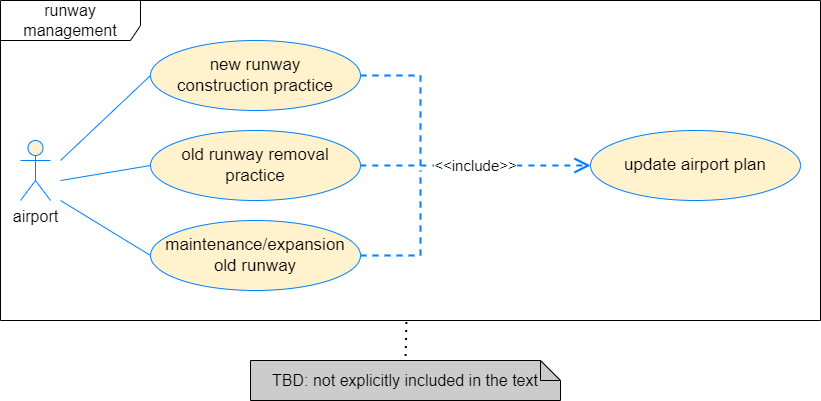
\includegraphics[scale=0.375]{figure8.png}
    \caption{Use case management runways, high summary abstraction level}
    \label{fig:enter-label}
\end{figure}
\bigbreak

\bigbreak
\begin{figure}[H]
    \centering
    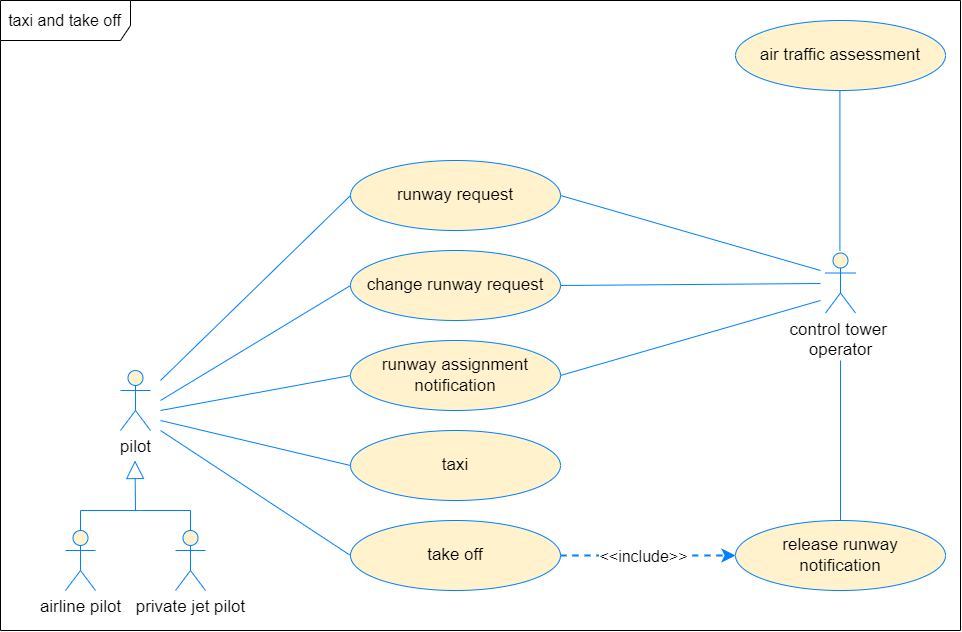
\includegraphics[scale=0.325]{figure9.png}
    \caption{Use case taxi and take off, high summary abstraction level}
    \label{fig:enter-label}
\end{figure}
\bigbreak

L'\textit{Activity Diagram} che segue è riferito solo al caso d'uso rappresentato in \textbf{Figure 9}.

\bigbreak
\begin{figure}[H]
    \centering
    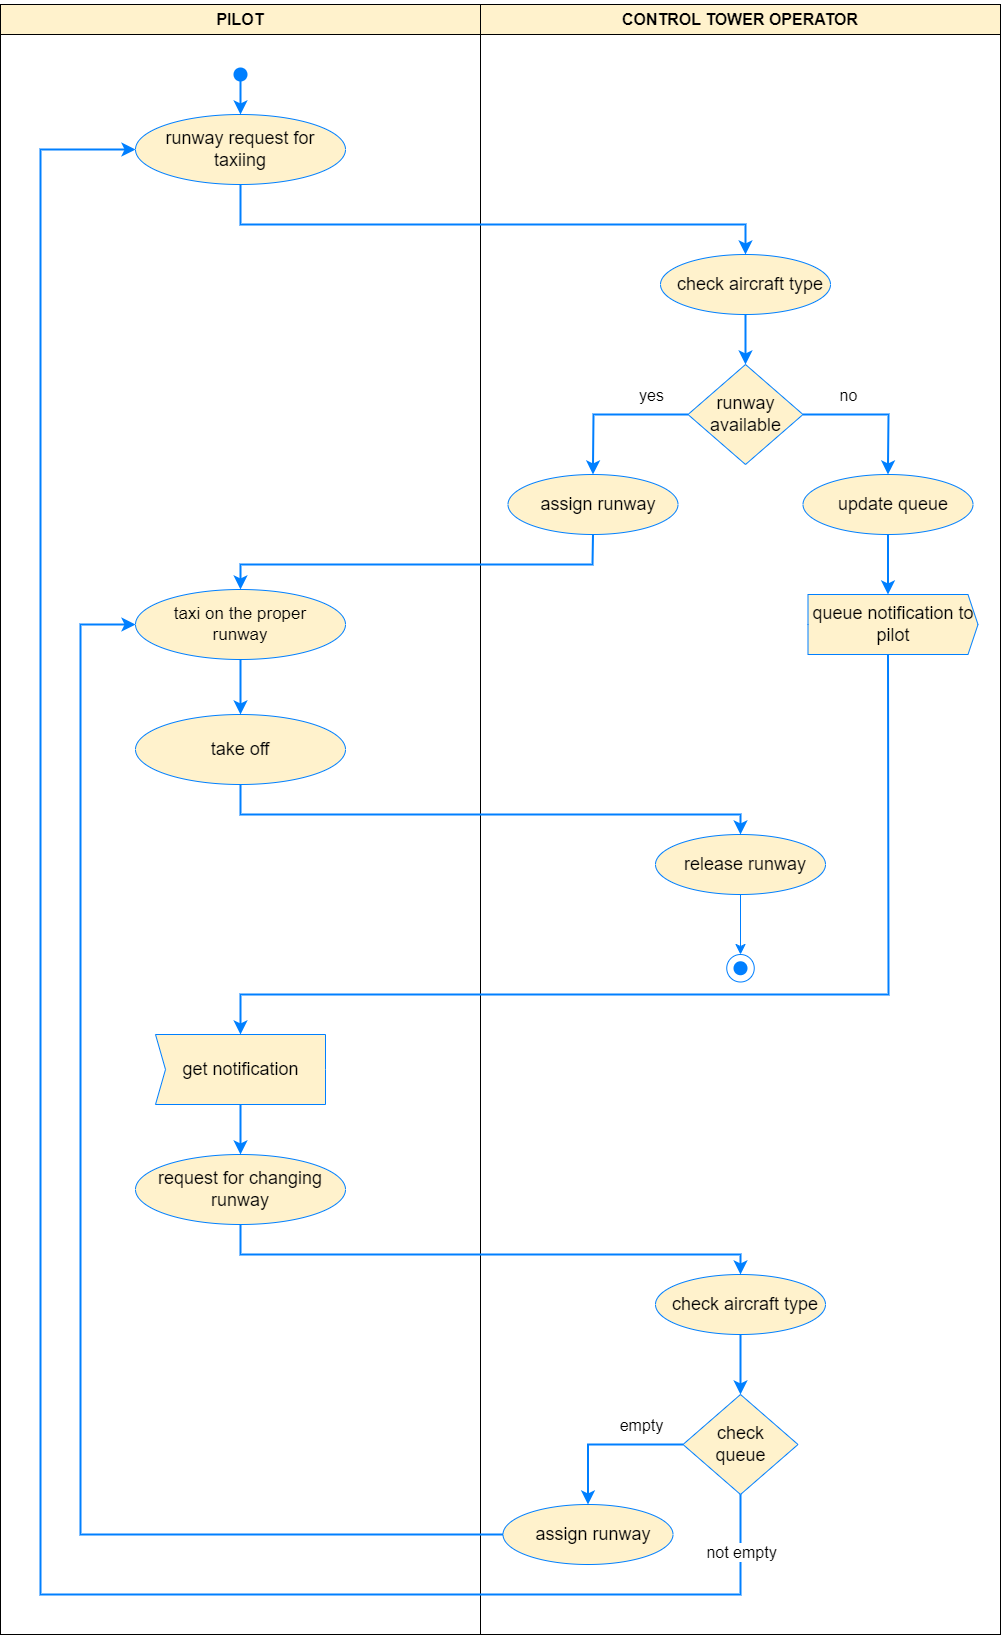
\includegraphics[scale=0.32]{figure10.png}
    \caption{Activity Diagram}
    \label{fig:enter-label}
\end{figure}
\bigbreak

\bigbreak
\begin{figure}[H]
    \centering
    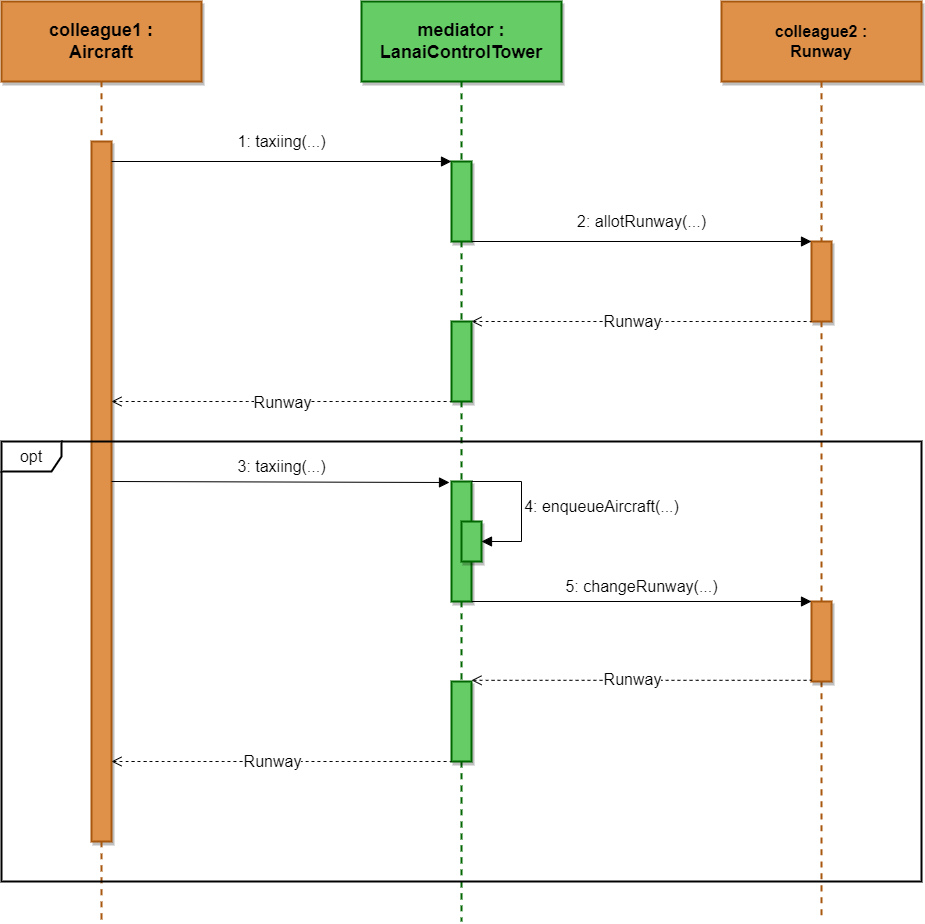
\includegraphics[scale=0.32]{figure11.png}
    \caption{Sequence Diagram}
    \label{fig:enter-label}
\end{figure}
\bigbreak

\textit{Note: Il sequence diagram riportato in \textbf{Figure 11} presenta un frame denominato "opt" la quale funzione è quella di indicare una particolare sequenza che si verificherà solo sotto certe condizioni. Modella in un certo senso la logica "se poi...".}


\section{Conclusioni}
In conclusione, l'elaborato ha fornito un'approfondita analisi e progettazione di un modello di dominio basato su un pattern specificamente scelto per affrontare uno scenario reale rappresentativo. Durante l'analisi, sono stati evidenziati chiaramente i vantaggi del pattern selezionato in relazione al contesto da modellare, sottolineando l'importanza degli strumenti di analisi utilizzati in fase di progettazione.

\bigbreak

La progettazione della struttura del modello è stata eseguita con la massima attenzione, mettendo in luce i partecipanti chiave e le relazioni che sussistono tra di essi. Questa fase di progettazione ha gettato le basi per l'implementazione pratica del modello.

\bigbreak

Nella sezione dedicata all'implementazione, sono stati forniti frammenti di codice che illustrano in modo chiaro e dettagliato gli aspetti salienti dello schema. Inoltre, sono stati definiti casi di test utilizzando JUnit per garantire che il modello funzioni correttamente in uno scenario che ne caratterizza l'intento.

\bigbreak

In sintesi, questo elaborato ha dimostrato una solida comprensione del modello di dominio scelto, evidenziando come esso sia applicabile in un contesto reale. L'approfondita analisi, la meticolosa progettazione e l'implementazione accurata con casi di test forniscono una base solida per la futura applicazione di questo modello, contribuendo al progresso e alla comprensione del dominio trattato. Inoltre, l'elaborato sottolinea l'importanza di un approccio strutturato e ben pianificato nella progettazione di modelli di dominio complessi. La chiara identificazione dei partecipanti e delle relazioni, insieme all'utilizzo di strumenti come JUnit per la verifica, dimostra un impegno verso la qualità e l'affidabilità del modello.

\bigbreak

Da un punto di vista più ampio, questo lavoro fornisce un contributo significativo alla comprensione del dominio specifico trattato. Gli aspetti analitici evidenziati nell'analisi complessiva suggeriscono che il pattern selezionato è appropriato per risolvere le sfide specifiche del contesto, aprendo la strada a futuri sviluppi e applicazioni nel settore.

\bigbreak

In conclusione, l'elaborato rappresenta un esempio eccellente di come l'analisi, la progettazione e l'implementazione accurata di un modello di dominio possano portare a soluzioni robuste e efficaci per problemi complessi. Questo lavoro costituirà una risorsa preziosa per chiunque sia interessato a esplorare ulteriormente il dominio e implementare soluzioni basate su questo pattern, contribuendo così al progresso nella comprensione e nell'applicazione di questo importante campo.

\end{sloppy}

\end{document}
